
\chapter{État de l'art}
\label{sec:state-art}


\chapterintro

.
\commentGP{TODO}


\section{Combinaisons d'analyses statiques et d'analyses dynamiques}
\label{sec:combinaison}


Les méthodes statiques et les méthodes dynamiques ont des avantages et des
inconvénients complémentaires : l'analyse statique étant complète mais
imprécise, l'analyse dynamique étant précise mais incomplète. L’idée de les
combiner pour associer leurs avantages et combattre leurs inconvénients
\cite{Ernst/WODA03} est une voie de recherche active et fructueuse dans le
domaine de la vérification de programmes.


\subsubsection*{\textsc{Static ANalysis and TEst}}

La méthode \sante \cite{Chebaro/11, \citesante}, mise en \oe{}uvre au sein de
\framac, combine l'interprétation abstraite, le {\em slicing} et la
génération de tests structurels avec \pathcrawler. L’analyse statique
signale les instructions risquant de provoquer des erreurs à l’exécution par des
alarmes, dont certaines peuvent être de fausses alarmes, puis l’analyse
dynamique génère des tests confirmant ou infirmant ces alarmes. Sur des
programmes de grande taille, l'analyse dynamique peut manquer de temps pour
classer toutes ces alarmes (à cause de l'explosion combinatoire des exécutions
possibles). Le {\em slicing} est utilisé pour réduire la taille des programmes
testés et donc le temps nécessaire à leur analyse.

Cette méthode utilise l'analyse de valeurs
(interprétation abstraite) afin de sélectionner les instructions pour lesquelles
le risque d'une erreur à l'exécution n'est pas écarté (nous les appellerons
``alarmes'' par la suite), par exemple une division par zéro ou un accès
invalide à la mémoire.

Ces alarmes vont être validées par des tests. Nous utilisons
\pathcrawler \cite{\citepathcrawler}, un outil de génération de tests
structurels, pour tenter de mettre en évidence un cas de test pour lequel le
chemin d'exécution passe par cette alarme, et provoque une erreur.

Pour diminuer le coût de la génération de tests, nous simplifions
syntaxiquement les programmes qui lui seront soumis pour ne garder que les
instructions dont dépend l'alarme considérée, on appelle cette opération
{\em slicing} \cite{Korel/88}. Nous obtenons ainsi des programmes plus simples,
tels que si une alarme est présente dans le programme d'origine, elle l'est
également dans les programmes simplifiés si le {\em slicing} a été paramétré
pour conserver les instructions dont dépend cette alarme. Et si elle provoque
une erreur dans le programme d'origine, alors il en sera de même dans les
programmes simplifiés, avec les mêmes entrées. L'utilisation du {\em slicing}
peut être paramétrée par différentes options, qui seront détaillées plus bas.

La première phase de la méthode (l'interprétation abstraite) peut donc assurer
que certaines instructions ne provoqueront pas d'erreur à l'exécution, tandis
que la seconde phase permet de confirmer que certaines alarmes produisent
effectivement une erreur à l'exécution. Et la mise en commun des résultats des
deux phases permet de classifier davantage d'alarmes dans l'une ou l'autre de
ces deux catégories que chacune des deux méthodes prise séparément. La preuve de
la correction de cette méthode et le résultat des analyses comparées sont
détaillés dans \cite{Chebaro/11} et \cite{\citesante} et ne seront pas répétés
ici.

L'option {\em none} signifie l'absence de {\em slicing} : le programme n'est pas
simplifié et est soumis en l'état à \pathcrawler.

L'option {\em all} génère un seul programme
simplifié contenant toutes les alarmes signalées par l'analyse de valeur. Cette
option ne tire pas profit du fait que certaines alarmes peuvent être
indépendantes (et peuvent donc être soumises séparément), la complexité du
programme soumis à \pathcrawler peut l'empêcher de générer des cas de
test pour toutes les alarmes dans le temps qui lui est imparti.

L'option {\em each} tente de corriger ce
défaut, elle génère un programme simplifié par alarme et invoque
\pathcrawler autant de fois. Ainsi, les alarmes les plus simples ne sont
pas pénalisées par les plus complexes. Néanmoins, en cas de dépendances
mutuelles entre alarmes, plusieurs programmes identiques seront soumis à
\pathcrawler, ce qui est une perte de temps.


L'option {\em min} tente de corriger
les inconvénients de {\em all} et de {\em each} et propose de générer une
couverture minimale des alarmes par {\em slicing}, de manière à regrouper dans
un même ensemble les alarmes ayant une relation de dépendance \cite{\citesante}.
Considérons par exemple les alarmes $\{a_1; a_2; a_3; a_4; a_5\}$, dont les
dépendances (Fig.~\ref{fig:deps}) sont : $a_2$ dépend de $a_1$; $a_5$ dépend de
$a_4$ qui dépend de $a_3$, qui dépend de $a_1$.
Dans cet exemple, la couverture minimale est constituée des deux ensembles
couvrants $\{a_1; a_2\}$ et $\{a_1; a_3; a_4; a_5\}$.


\begin{figure}
  \centering
  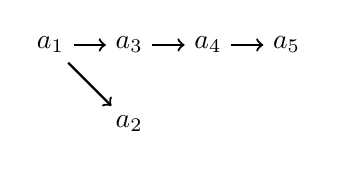
\begin{tikzpicture}
    \node(s) at (0,1) {$a_1$};
    \node(t) at (1,0) {$a_2$};
    \node(q) at (1,1) {$a_3$};
    \node(d) at (2,1) {$a_4$};
    \node(v) at (3,1) {$a_5$};
    \path[->,thick] (s) edge (q);
    \path[->,thick] (q) edge (d);
    \path[->,thick] (d) edge (v);
    \path[->,thick] (s) edge (t);
  \end{tikzpicture}
  \caption{Graphe de dépendances des alarmes}
  \label{fig:deps}
\end{figure}


Chacun de ces ensembles sera utilisé pour générer un programme simplifié ne
contenant que des alarmes ayant une relation de dépendance, évitant ainsi
d'avoir plusieurs programmes identiques en cas de dépendances mutuelles (et
réduisant le nombre d'appels à \pathcrawler).
On remarque que si toutes les alarmes sont dépendantes, on se retrouve dans le
cas de {\em all}, et si elles sont toutes indépendantes, on se retrouve dans le
cas de {\em each}.

Dans le cas où les ensembles couvrants contiennent de nombreuses alarmes,
{\em min} hérite de l'inconvénient de l'option {\em all} : les alarmes les plus
complexes à classifier pénalisent les autres, qui peuvent ne pas être
diagnostiquées dans le temps imparti.

Pour corriger ce défaut, l'option {\em smart} est définie.
Elle consiste à appliquer {\em min} itérativement en
diminuant l'ensemble des alarmes considérées à chaque itération. Les alarmes
supprimées seront des alarmes classifiées ou des {\em alarmes finales}.
Nous appelons \emph{alarme finale} une alarme dont aucune autre alarme de dépend
mais pouvant avoir des dépendances mutuelles avec d'autres alarmes finales.
Sur notre exemple, $a_2$ et $a_5$ sont des alarmes finales (sans dépendances
mutuelles).

De cette manière, le {\em slicing} appliqué à l'itération suivante (sur
l'ensemble des alarmes privé des alarmes finales) produira un programme
simplifié plus petit. Ainsi, les alarmes qui n'ont pas été diagnostiquées à
l'itération précédente auront une chance supplémentaire de l'être, et ainsi de
suite jusqu'à ce que toutes les alarmes soient diagnostiquées ou que l'ensemble
considéré soit vide.

Sur l'exemple considéré plus haut, la première itération génère la
couverture minimale $\{\{a_1; a_2\}; \{a_1; a_3; a_4; a_5\}\}$. S'il reste des
alarmes non diagnostiquées, les alarmes finales ($a_2$ et $a_5$) et les alarmes
diagnostiquées ne seront plus considérées. L'itération suivante génère la
couverture $\{\{a_1; a_3; a_4\}\}$. Et ainsi de suite.


\subsubsection*{\dyta}


\dyta \cite{\citedyta} est un outil combinant une phase d'analyse statique et
une phase d'analyse dynamique. \codecontracts \cite{\citecodecontracts} est
utilisé pour spécifier des pré/post-conditions et des invariants de programmes
C\#, il identifie également les bugs potentiels (violations de contrat) par
interprétation abstraite.

\dyta instrumente ensuite le programme pour rajouter des instructions
assurant le rôle de pré-conditions, pour ne pas générer de cas de test qui n'ont
aucune chance de produire d'erreur à l'exécution. L'instrumentation rajoute
également des points de contrôle à l'endroit des instructions signalées par
l'analyse statique, afin de guider l'exécution symbolique dynamique du programme
par \pex. Cette étape est semblable à l'instrumentation
opérée par \sante pour rajouter des points de contrôle afin
de guider l'exécution concolique du programme par \pathcrawler.

L'analyse statique du graphe du flot de contrôle du programme permet à
\dyta de calculer les points de contrôle à partir desquels les alarmes
(instructions potentiellement dangereuses) sont inatteignables. La génération
dynamique de tests réduit le nombre de faux positifs de l'analyse statique, et
cette dernière guide l'exploration pour la génération dynamique de tests.


\subsubsection*{Vérification collaborative et test}


Cette méthode \cite{Christakis/FM12} part du constat que la plupart
des outils de vérifications statiques (outils utilisant simplement des
heuristiques, outils d'interprétation abstraite, model-checkers, ou outils de
preuve) font des compromis afin d'améliorer les performances, de réduire le
nombre de faux positifs ou de limiter l'effort à fournir pour annoter le
programme. Cela se traduit par la supposition d'une propriété tout au long de
l'analyse dy programme (par exemple qu'un certains type d'erreurs ne peut pas
se produire), cette propriété n'est pas vérifiée par l'analyseur. Ceci
implique que de tels analyseurs ne peuvent garantir l'absence d'erreurs dans un
programme. Si un analyseur fait un compromis en supposant une propriété, il
faut utiliser un autre analyseur capable de valider cette propriété.

Cette méthode propose d'exprimer les compromis dans un langage de contrats,
afin de faciliter la collaboration entre plusieurs outils d'analyse statique
et permettant de décrire le fait qu'un assertion ait été complètement vérifiée
par un analyseur ou partiellement vérifiée sous certaines hypothèses.

Pour faciliter la vérification statique du programme, l'utilisateur doit au
préalable ajouter des annotations (invariants de boucle par exemple). Les
propriétés qui n'ont pas été vérifiées statiquement sont validées par des tests
unitaires. Le programme est instrumenté afin de rajouter des vérifications à
l'exécution pour guider la génération de contre-exemples. \pex est utilisé pour
générer des cas de test par exécution concolique,
mettant en évidence des contre-exemples. L'utilisateur peut décider de
privilégier l'analyse statique ou le test selon qu'il spécifie ou non son
programme.

Cette combinaison d'analyse statique, d'une instrumentation et du test est
comparable à \sante, bien qu'il manque l'étape de slicing
qui permet à \sante d'économiser du temps sur l'analyse dynamique. En
revanche, cette méthode présente l'avantage de combiner plusieurs analyseurs
statiques et de vérifier partiellement des propriétés, ce qui n'est pas encore
possible avec \sante.


\subsubsection*{Vérification de propriétés décrites par des automates finis}


Cette méthode \cite{Slaby/FMICS12} combine une instrumentation du
code source, une étape de {\em slicing} et une exécution symbolique.
L'instrumentation rajoute des instructions simulant le comportement de
l'automate fini correspondant au programme, dont les états correspondent aux
propriétés du programme à vérifier.
Le {\em slicing} est appliqué pour réduire la taille du programme, on ne
conserve que le code relatif aux états d'erreur de l'automate. Le programme
simplifié doit être équivalent au programme instrumenté en ce qui concerne
l'atteignabilité des états d'erreur de l'automate.
L'exécution symbolique du programme par \klee \cite{\citeklee} va permettre
de mettre en évidence des contre-exemples pour ces propriétés.

L'utilisation du {\em slicing} afin de réduire la portion de code analysée
(et donc le nombre de chemins d'exécution) par l'exécution symbolique est
similaire à \sante \cite{\citesante}. En revanche, cette méthode ne semble
pas applicable quel que soit le type d'erreur.
\cite{Slaby/FMICS12} prend l'exemple de verrous à poser sur des
variables du programme. L'instrumentation repère des motifs bien précis dans le
programme et le code généré est spécifique à ce type d'erreur. Contrairement à
\sante, cette méthode n'applique pas d'analyse statique plus générale
(pouvant lever différents types d'alarmes) avant l'instrumentation.


\subsubsection*{Localisation d'erreurs par slicing guidé par la trace d'exécution}


Cette méthode \cite{Jiang/QSIC12} utilise un {\em slicing} arrière à
partir d'une instruction de déréférencement produisant une {\em Null Pointer
Exception} (en Java). Le {\em slicing} est guidé par la trace du programme
fournissant la pile des appels de méthode n'ayant pas terminé. Une analyse
statique des pointeurs est ensuite opérée sur le programme slicé afin de
déterminer si chacun des pointeurs peut être \lstinline[language=java]{null}.
Puis une analyse d'alias est opérée afin d'augmenter la précision de l'analyse
statique.

%% Contrairement à \sante qui commence par utiliser une
%% analyse statique, dont le résultat paramètre le {\em slicing}, puis termine par
%% une analyse dynamique; cette méthode commence par une analyse dynamique, dont
%% le résultat paramètre le {\em slicing}, puis termine par une analyse statique.


\subsubsection*{\cegar : Raffinement d'abstraction guidé par des contre-exemples}


Le raffinement d'abstraction guidé par des contre-exemples \cite{\citecegar}
associe
l’abstraction par prédicats et le model-checking : une abstraction du programme
est générée à partir d’un ensemble de prédicats et invariants. Si le
model-checking prouve la non-accessibilité des états d'erreurs de l'automate,
alors le modèle concret est correct (pas d'erreurs de sûreté ou de liveness).
Si le model-checking a trouvé un contre-exemple pour le modèle abstrait il faut
déterminer s'il correspond à un contre-exemple réel dans le système concret.
Pour cela, l'algorithme détermine s'il existe une trace d'exécution concrète
correspondant à la trace d'exécution abstraite aboutissant au contre-exemple.
Si une telle trace existe, un bug a été trouvé. Sinon, de nouveaux prédicats
seront créés pour raffiner l'abstraction afin que ce contre-exemple en soit
absent à la prochaine itération. Et ainsi de suite. Ce processus peut ne pas
terminer. Plusieurs outils de vérification se basent sur cette méthode, parmi
lesquels \blast \cite{\citeblast}, \magic \cite{\citemagic} et
\slam \cite{\citeslam}.

Cette approche élimine les contre-exemples un par un, l'abstraction ainsi
générée peut donc mettre un certain temps avant de converger vers une forme
acceptable. Une amélioration a été proposée afin d'accélérer la convergence du
raffinement de l'abstraction : \cegaar \cite{\citecegaar}. Cette technique
élimine une infinité de contre-exemples (traces infaisables) de la forme
$\alpha . \lambda^{*} . \beta$ en une seule étape, où $\lambda$ correspond à une
ou plusieurs exécutions d'une boucle.


\subsubsection*{\blast}


\blast \cite{\citeblast} vérifie les propriétés temporelles de sûreté d'un
programme C, ou met en évidence un chemin d'exécution violant une propriété. Le
raffinement des abstractions du programme est basé sur une abstraction par
prédicat et la découverte des prédicats se fait par interpolation. C'est une
implémentation de la méthode \cegar \cite{\citecegar} tout comme
\slam \cite{\citeslam} et \magic \cite{\citemagic}. La génération des cas
de test se fait par exécution symbolique.

\blast ne traite ni les débordements arithmétiques ni les opérations
bit-à-bit, et considère que toutes les opérations arithmétiques sur les
pointeurs sont sûres. Le langage d'invariants utilisé pour décrire les
propriétés ne contient pas de quantificateurs, contrairement à \acsl.


\subsubsection*{\smart}


\smart \cite{\citesmart} (basé sur son prédécesseur \dart \cite{\citedart})
génère des tests par exécution concolique. Pour résoudre le problème de
l'explosion du nombre de chemins, il va calculer à la demande des résumés de
fonction qui sont des pré-conditions et post-conditions pour chaque fonction
(contraintes sur les variables en entrée et en sortie). Ces résumés vont être
réutilisés si possible afin d'éviter de ré-exécuter la fonction correspondante.
La génération automatique de ces résumés est présentée comme se faisant par
``analyse statique interprocédurale'' mais se rattacherait plutôt à une analyse
dynamique car utilisant une exécution symbolique (et résolution de contraintes).
\smart exécute une analyse dynamique compositionnelle, c'est-à-dire que les
résultats intermédiaires sont mémorisés sous la forme de résumés réutilisables.
C'est une extension de l'algorithme d'analyse dynamique non compositionnelle de
\dart, mais n'effectue pas d'analyse statique. 


\subsubsection*{\synergy, \dash et \yogi}


\synergy \cite{\citesynergy} est un algorithme combinant du test (essayer
d'atteindre un état d'erreur) et une abstraction (trouver une abstraction
suffisamment précise montrant qu'aucun chemin ne peut atteindre un état
d'erreur). La sous-approximation du test et la sur-approximation de
l'abstraction sont raffinées de manière itérative. L'abstraction est utilisée
pour guider la génération de tests. Les tests sont utilisés pour décider
{\em où} raffiner l'abstraction.
Les états de l'abstraction, les régions, sont des classes d'équivalence des
états du programme concret. S'il n'existe aucun chemin de la région initiale
vers une région d'erreur, alors il n'existe aucune suite de transitions
concrètes menant d'un état initial concret à un état d'erreur concret.

\dash \cite{\citedash} est une évolution de \synergy, prenant en
compte les appels de procédure et les pointeurs (contrairement à
\synergy).
\dash est inter-procédural mais non compositionnel.
\dash raffine l'abstraction en utilisant uniquement
les relations d'alias mises en évidence par les tests. La génération de tests
guide non seulement {\em où} raffiner l'abstraction, mais aussi {\em comment}
la raffiner. Cet algorithme est implémenté dans \yogi \cite{\citeyogi}.
\synergy combine \slam et \dart (\cegar compositionnel + test non
compositionnel). L'algorithme est intra-procédural.


\subsubsection*{\Smash}


\Smash \cite{\citesmash} combine une abstraction par prédicats et une génération
dynamique de tests (par exécution concolique). Pour chaque fonction, un résumé
est calculé par analyse statique (vrai pour toutes les exécutions, permettant
de prouver l'absence d'erreurs, c'est une sur-approximation) et un autre résumé
est calculé par analyse dynamique (vrai pour quelques exécutions uniquement,
permettant de montrer l'existence d'erreurs, c'est une sous-approximation). Ces
résumés sont calculés à la demande et seront utilisés aussi bien par l'analyse
statique que par l'analyse dynamique (les deux analyses s'exécutent
simultanément).
Ces résumés sont progressivement raffinés pour chaque fonction, afin de prouver
qu'une propriété n'est jamais violée (si un résumé statique est applicable), ou
de mettre en évidence une exécution violant une propriété (si un résumé
dynamique est applicable). Par construction, il n'est pas
possible que les deux résumés soient applicables.
\Smash est la version compositionelle de \dash.

La figure~\ref{tab:microsoft-summary} résume les caractéristiques de ces outils.

\begin{figure}[bt]
  \centering
  \begin{scriptsize}
    \begin{tabular}{c|c|c|c|c|c|c}
      \multirow{3}{*}{Outils} & \multicolumn{3}{c|}{Analyse statique}
      & \multicolumn{3}{c}{Analyse dynamique} \\
      & \multirow{2}{*}{intra-proc} & \multicolumn{2}{c|}{inter-proc}
      & \multirow{2}{*}{intra-proc} & \multicolumn{2}{c}{inter-proc} \\
      & & non-compo & compo & & non-compo & compo \\
      \hline
      \slam & & & \ok & & & \\
      \hline
      \dart & & & & & \ok & \\
      \hline
    \smart & & & & & & \ok \\
    \hline
    \synergy & \ok & & & \ok & & \\
    \hline
    \dash & & \ok & & & \ok & \\
    \hline
    \Smash & & & \ok & & & \ok \\
    \end{tabular}
  \end{scriptsize}
  \caption{Type d'analyse et caractéristiques des outils de Microsoft}
  \label{tab:microsoft-summary}
\end{figure}


\subsubsection*{Analyses statique et dynamique pour la génération d'invariants}


Cette méthode \cite{Gupta/TACAS09} propose une solution au problème du
passage à l'échelle de la génération d'invariants (de programmes impératifs) par
résolution de contraintes. Les invariants arithmétiques linéaires sont générés
d'après les informations obtenues par interprétation abstraite du programme, par
exécution concrète et par exécution symbolique du programme. Ces informations
permettent de générer des contraintes qui vont permettre au solveur de
contraintes de simplifier le système de contraintes et de réduire l'espace de
recherche.


\subsubsection*{\dsdcrasher et \checkncrash}


L'outil \dsdcrasher \cite{\citedsdcrasher} combine une première analyse
dynamique, une analyse statique et une seconde analyse dynamique. La première
analyse dynamique utilise une génération de tests et des techniques
d'apprentissage pour générer des invariants probables (inférence de la
spécification par \daikon \cite{\citedaikon}).

Les deux dernières étapes sont celles de l'outil \checkncrash
\cite{\citecheckncrash}. L'analyse statique (\escjavatwo \cite{\citeescjavatwo})
va émettre des alarmes concernant le non-respect des invariants, et la seconde
analyse dynamique va tenter de confirmer ces alarmes par résolution de
contraintes et génération de tests (\jcrasher \cite{\citejcrasher}). La
classification des alarmes et la génération de tests sont très dépendantes de
la qualité des invariants générés par \daikon.

Cette méthode se distingue de \sante \cite{\citesante} par son analyse
dynamique préliminaire qui détecte des invariants afin de guider l'analyse
statique. En revanche, elle n'utilise pas le {\em slicing} qui permet
d'augmenter le taux de classification des alarmes par l'analyse dynamique.


\subsubsection*{Génération de données de test par algorithme génétique}


\cite{Romano/ICST11} propose une méthode de génération de données
de test mettant en évidence des {\em Null Pointer Exceptions} de Java. Tout
d'abord une analyse inter-procédurale du flot de contrôle et du flôt de données
collecte les chemins menant aux exceptions. Cette analyse se fait en arrière, en
partant des exceptions, propageant les contraintes sur les entrées dans le CFG.
Les entrées de test sont ensuite générées par un algorithme génétique, dans le
but de couvrir ces chemins. Les individus (des entrées potentielles), dont le
type de donnée peut être complexe, sont encodés sous forme XML.

Cette méthode a été comparée avec d'autres façons de générer des données de
test \cite{Ahn/TAP10}, leurs expérimentations
ont montré qu'elle était plus efficace que d'autres stratégies de recherche
optimale comme le {\em hill climbing} et le recuit simulé, mais est moins
efficace que la programmation par contraintes (en terme de temps d'exécution). 


\subsubsection*{Génération de tests unitaires à partir de preuves formelles}


\cite{Engel/TAP07} présente une méthode de
génération automatique de tests unitaires pour \textsc{Java Card} à partir d'une
tentative de preuve formelle du système, qui doit être au préalable annoté en
utilisant le langage de spécification \jml \cite{\citejml}.

L'information contenue dans la preuve (même partielle) est utilisée
pour extraire des données de test à partir des conditions de chemins. Les
oracles sont générés à partir des postconditions. En revanche, il n'y a aucune
garantie sur le critère de couverture des chemins par les tests générés,
celle-ci dépend de la qualité de la spécification du code (présence des
invariants de boucle, etc.).


\section{Aide à la preuve de programmes}


\commentGP{TODO}
état de l'art ISSRE'15


\section*{Conclusion du chapitre}


\commentGP{TODO}
